\documentclass[
 paper=A4,pagesize=automedia,fontsize=12pt,
 BCOR=15mm,DIV=22,
 twoside,headinclude,footinclude=false,
 ngerman,fleqn,             % fleqn = linksbündige Ausrichtung von Formeln
 bibtotocnumbered,          % Literaturverz. im Inhaltsverz. eintragen
 liststotoc,                % Abbildungsverz. im Inhaltsverz. eintragen
 listsleft,                 % Abbildungsverz. an der längsten Nummer ausrichten
 pointlessnumbers,          % kein Punkt nach Überschriftsnummerierung
 cleardoublepage=empty      % Vakatseiten ohne Paginierung
]{scrbook}
\setlength\parindent{0em}

% Kodierung, Schrift und Sprache auswählen
\usepackage[utf8]{inputenc}
\usepackage[T1]{fontenc}
\usepackage[english]{babel}
% damit man Text aus dem PDF korrekt rauskopieren kann
\usepackage{cmap}
% Layout: Kopf-/Fußzeilen, anderthalbfacher Zeilenabstand
\usepackage{scrpage2} \pagestyle{scrheadings}
                      \clearscrheadfoot
                      \ihead{\headmark}\ohead{\pagemark}
                      \automark[subsection]{section}
                      \setheadsepline{0.5pt}
\usepackage{setspace} \onehalfspacing
\deffootnote{1em}{1em}{\textsuperscript{\thefootnotemark }}
% Grafiken, Tabellen, Mathematikumgebungen
\usepackage{graphicx,xcolor}
\usepackage{tabularx}
\usepackage{amsmath,amsfonts,amssymb}
% Darstellung von Fließumgebungen
\usepackage{flafter,afterpage}
\usepackage[section]{placeins}
\usepackage[margin=8mm,font=small,labelfont=bf,format=plain]{caption}
\usepackage[margin=8mm,font=small,labelfont=bf,format=plain]{subcaption}

\numberwithin{equation}{chapter}
\numberwithin{figure}{chapter}
\numberwithin{table}{chapter}

%%%%%%%%%%%%%%%%%%%%%%%%%%%%%%%%%%%%%%%%%%%%%%%%%%%%%%%%%%%%%%%%%%%%%%%%%%%%%%%%
% Ab hier ist Platz für eigene Ergänzungen (Pakete, Befehle, etc.)

% Dieses Paket liefert den Blindtext, der als Platzhalter in den Beispieldateien steht.
% Das kannst Du also entfernen, wenn Du den Blindtext nicht mehr brauchst.
\usepackage{lipsum}

% workaround
\makeatletter\def\set@pdftextpagesize{\set@pdftexpagesize}\makeatother

\usepackage[backend=bibtex]{biblatex}
\usepackage{hyperref}

\bibstyle{nat}
\bibliography{sources}

\makeatletter
\newcommand{\Spvek}[2][r]{%
  \gdef\@VORNE{1}
  \left(\hskip-\arraycolsep%
    \begin{array}{#1}\vekSp@lten{#2}\end{array}%
  \hskip-\arraycolsep\right)}

\def\vekSp@lten#1{\xvekSp@lten#1;vekL@stLine;}
\def\vekL@stLine{vekL@stLine}
\def\xvekSp@lten#1;{\def\temp{#1}%
  \ifx\temp\vekL@stLine
  \else
    \ifnum\@VORNE=1\gdef\@VORNE{0}
    \else\@arraycr\fi%
    #1%
    \expandafter\xvekSp@lten
  \fi}
\makeatother

\usepackage{multirow}
\usepackage{longtable}
\usepackage{pdfpages}


\begin{document}

% \frontmatter
\mainmatter


% Titelpageseite
\begin{titlepage}
 \begin{tabularx}{\linewidth}{X}
  
\includegraphics[width=6cm]{TU_Logo_SW} \\\hline\hline

  \vspace{4.5em}

  \begin{singlespace}\begin{center}\bfseries\Huge
  
  Partial decay widths and form factor implementation
  for the simulation of the \(\Lambda_c^+\) decays in SHERPA
  
  \end{center}\end{singlespace}

  \vspace{5.5em}

  \begin{singlespace}\begin{center}\large
   Bachelor-Arbeit \\ zur Erlangung des Hochschulgrades \\ 
   Bachelor of Science \\ 
   im Bachelor-Studiengang Physik
  \end{center}\end{singlespace}\medskip

  \begin{center}vorgelegt von\end{center}
  \begin{center}
   {\large Sven Schiffner} \\ geboren am 28.10.1994 in Sebnitz
  \end{center}\medskip

  \begin{singlespace}\begin{center}\large
   Institut für Kern- und Teilchendphysik \\
   Fachrichtung Physik \\
   Fakultät Mathematik und Naturwissenschaften \\
   Technische Universität Dresden \\ 2017
  \end{center}\end{singlespace}
 \end{tabularx}
\end{titlepage}


% Gutachterseite
\thispagestyle{empty}\vspace*{48em}

Eingereicht am 24.~Mai~2017\vspace{1.5em}
\par{\large\begin{tabular}{ll}
 1. Gutachter: & Dr.~Frank Siegert \\
 2. Gutachter: & Prof.~Dr.~Michael Kobel \\
\end{tabular}}


% Abstractseite
\newpage
\begin{center}\large\bfseries Summary\end{center}


Abstract \\ 
English: \\

\vspace{20em}
Abstract \\ 
Deutsch \\
 
 
% Inhaltsverzeichnis

%\cleardoublepage
\tableofcontents



% Hauptteil

\chapter{Introduction}
One of the big questions of mankind is, why are we here. And the correspondending 
question is in physics is, why exists more matter than anti-matter in the universe. 
This thesis can't clear the question but it can be a part of the big picture.\\
The \texttt{LHC} (Large Hadron Collider) is one of the biggest experiments of 
humanity. This accelerator collides proton with protons, lead nuclei with 
protons or lead nuclei with lead nuclei. One detector of this big apparatus 
is the \texttt{LHCb}. The \texttt{LHCb} is a try to find the answer of the 
above question. It examines assymetries in the decay of matter and 
anti-matter mainly for lead-lead-collissions. And so deviations 
from the Standard Model. The Standard Model is a theory that describes the 
fundamental interactions between and the elementary particles itself very 
well. These deviations can result in additions to the Standard Model to consider 
a asymmetry between matter and anti-matter. And so lead to an answer for the 
matter surplus.\\
For this the results from the experiment has to be compared to the 
theoratical results. But simulations are needed for the theoratical results. 
This comes from the different interactions that happens through a particle 
collision. A lot of particles are created and decay. On of the simulation 
tools is \texttt{Sherpa}. This program use Monte-Carlo techniques to obtain 
results.\\
One possible baryon that can be created is the \(\Lambda_c^+\). It is the 
lightest baryon that contains a charm quark. The charm quark is like the 
up quark that builds together with the down quark neutrons and protons but 
heavier.\\
For a good comparison between the experimental results and the theoratical 
simulations is it important to implement as much particles in the simulation 
as possible. This leads in a better description of the reaction and so in better 
theoretical results.
\par
This thesis has the goal to improve the simulation through a better implementation 
of the \(\Lambda_c^+\) decays.

\chapter{Basic Physical Principles}
\section{Baryons}
A baryon is a subatomic particle. It is composite and contains three quarks.
The baryons form together with the mesons the class of the hadrons. Mesons are 
composed of two quarks, one quark and one antii-quark.\\
Protons and neutrons which are the components of our normal matter are baryons. 
These are the lightest baryons. The proton is made of two up quarks and one down 
quark. The neutron contains two down quarks and one up quark.\\
All observed events so far feature that the number of baryons in a reaction is 
observed. To use this in calculations every quark get the baryon number \(B = 1/3\) and 
every anti-quark \(B = -1/3\). In a decay from a baryon (\(\sum B = 1\)) the final 
products has to be a baryon (\(\sum B = 1\)) or two baryons (\(\sum B = 2\)) 
and an anti-baryon (\(\sum B = -1\)) and so on. 

\subsection{\(\Lambda_c^+\) Baryon}
The \(\Lambda_c^+\) has a mass of \(2286.46 \pm 0.14 \text{MeV}^
{\text{\cite{lambda-pdg}}}\) and a mean life time of \(\left( 2.00 \pm 0.06\right)
\cdot 10^{-13} \text{s}^{\text{\cite{lambda-pdg}}}\). It is one of the lightest charmed 
baryons and is made of one up, down and charm quark. Its charge is +1 of the 
elementary charge\(^{\text{\cite{lambda-pdg}}}\).

\section{Decays}
Decays are processes with one particle in the initial state and n particles 
in the final state for n= 2,3,{\ldots}. The decayed particle must not be in the final 
state. This makes the difference to radiation processes. The decay process can 
always be transformed in to the rest mass frame of the decayer. So the mass 
of the particle in the inital state is a limit for the dynamic of the process.\\
A decay process or more general a transition process is characterized through 
Fermi's golden rule:
\begin{equation}
  \Gamma_{fi} = 2 \pi |T_{fi}|^2 \rho\left(E_i\right), \label{eq:fermi}
\end{equation}
where \(T_{fi}\) is the transition matrix element and 
\(\rho\left(E_i\right)\) is the density of states. The result is the transition 
rate \(\Gamma_{fi}\). In natural units the unit of the transition rate is \(\text{GeV}^{-1}\).\\
The \(\Gamma_{fi}\) is also called partial decay width. And is characteristic value 
of a decay process. The sum over all partial decay widths is called 
total decay width:
\begin{equation}
  \Gamma_i = \sum_f \Gamma_{fi}. \label{eq:total}
\end{equation}
The total width{\eqref{eq:total}} is an criterion for the lifetime of the 
decaying particle. The lifetime  of the particle in natural units is the 
inverse of \(\Gamma_i\):
\begin{equation}
  \tau_i = \frac{1}{\Gamma_i}. \label{eq:lifetime}
\end{equation}
The branching ratio is the probability to decay in a specific final 
state. It can be calculated with the partial and total decay width:
\begin{equation}
  BR( i \rightarrow f) = \frac{\Gamma_f}{\Gamma}. \label{eq:br}
\end{equation}

\section{Weak Decay}
A weak decay is the transition of a particle through the weak interaction. An 
elementary particle that is possibly part of an composite can in this 
way decay to a W\(^\pm\)-Boson and a correspondending particle. But the W-Boson only 
couple to lef-handed fundamental partciles and right-handed fundamental 
anti-particles. The spinor for the weak interaction than looks like 
{\eqref{eq:spinor}}. There the upper particle have isospin -1/2 and the lower isospin 
+1/2.
\begin{equation}
  \Spvek{\nu_e; e^-}_L,\Spvek{\nu_\mu; \mu^-}_L, \Spvek{s; c}_L, \Spvek{e^+; \bar{\nu}_e}_R, 
  \Spvek{\mu^+; \bar{\nu}_\mu}_R \text{ etc.} \label{eq:spinor}
\end{equation}
Above only the particles are shown that are relevant for this 
thesis.

\begin{figure}[h]
  \centering
  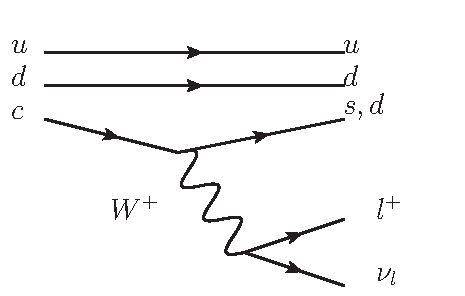
\includegraphics[page=1, width=0.5\textwidth]{semileptonic_lambdac+}
  \caption{Semileptonic decay modes of the \(\Lambda_c^+\) into a neutron (udd)
    or a \(\Lambda\) (uds), an positron or an anti-muon and the correspondending 
  neutrino (own graphic)}\label{fey:lambda}
\end{figure}

In the Feynman diagram {\ref{fey:lambda}} the semileptonic decay of a \(\Lambda_c^+\) 
is visible. The up and down quark from the \(\Lambda_c^+\) are unchanged. 
They can only influence the transition matrix element through a different 
behavior of the charm quark. The charm quark transforms through the weak 
decay in to a down or strange quark. The down quark forms with the other two 
qarks a neutron and the strange quark a \(\Lambda\). The emited W\(^+\)-Boson 
decays leptonic in an anti-lepton and the correspondending neutrino.
Other decays of the W\(^+\)-boson are possible. For this thesis only the 
semileptonic decays channels are relevant. The complete dynamic of the process 
will be discussed in {\ref{sec:v-a}}. In this section we will take a closer 
look at the W\(^\pm\) propagator.\\
The value for a W\(^\pm\) propagator is \(\frac{g_w^2}{8}\frac{1}{q^2 - m_W^2}\).
The transferred momentum is \(q^2 = \left(p_f - p_i\right)^2\). It is limited 
by the initial state mass and for most decays this is much less than the mass 
of the W\(^\pm\) boson. The last fraction can be approximated through 
\(-\frac{1}{m_W^2}\) for \(m_i \ll m_W\). The whole term becomes to \(-\frac{g_w^2}{8 m_W^2}\) 
and this is the Fermi coupling constant \(G_F\) except a factor \(-\frac{1}{sqrt{2}}\):
\begin{equation}
  \frac{G_F}{\sqrt{2}} = \frac{g_w^2}{8 m_W^2}. \nonumber
\end{equation}
The weak decay has in this approximation a threesome vertex with the coupling 
constant \(G_F\).

\section{V-A current} \label{sec:v-a}
The value of a vertex where two matching leptons transforms into a  
W\(^\pm\) boson is \(-i \frac{g}{2\sqrt{2}} \gamma^\mu\left(1-\gamma^5\right)\).
If the sum is splitted, the the term without \(\gamma^5\) is called vector and 
the part with the \(\gamma^5\) axial-vector through the geometrical effect of 
the \(\gamma\)-matrix. The transition from quarks needs an additional factor 
\(V_{if}\). i is the quark and in the initial state and f the quark in the 
final state. The factor comes from the CKM-matrix\(^{\text{\cite{ckm}}}\). The 
matrix from {\cite{ckm}} is
\begin{equation}
  V_{CKM} =
  \begin{bmatrix}
    0.97434^{+0.00011}_{-0.00012} &  0.22506 \pm 0.00050 & 0.00357 \pm 0.00015 \\
    0.22492 \pm 0.00050 & 0.97351 \pm 0.00013 & 0.0411 \pm 0.0013 \\
    0.00875^{+0.00032}_{-0.00033} & 0.0403 \pm 0.0013 & 0.99915 \pm 0.00005
  \end{bmatrix}. \label{eq:ckm}
\end{equation}
With the general Feynman rules for vertices and propagators the transition matrix 
element becomes to
\begin{equation}
  T = \frac{G_F}{\sqrt{2}} V_{Qq} \bar{u_l}\gamma^\mu\left(1 - \gamma^5\right) 
  u_{\nu_l} \langle B(p', s') | J_\mu | \Lambda_c(p, s) \rangle \label{eq:trans}
\end{equation}
ike in {\cite[Eq. 1]{Frank}}, where B in stands for the neutron or \(\Lambda\). The current 
\(J_\mu\) can be splitted in a vector and an axial-vector part \(J_\mu = V_\mu - 
A_\mu \) like in
\begin{align}
  \langle B(p', s') | V_\mu | \Lambda_c(p, s) \rangle & = \bar{u}(p', s') 
  \left( F_1(q^2) \gamma_\mu + F_2(q^2)\frac{p_\mu}{m_{\Lambda_c}} + 
  F_3(q^2)\frac{p'_\mu}{m_B} \right) u(p, s) \nonumber \\
  \langle B(p', s') | A_\mu | \Lambda_c(p, s) \rangle & = \bar{u}(p', s') 
  \left( G_1(q^2) \gamma_\mu + G_2(q^2)\frac{p_\mu}{m_{\Lambda_c}} + 
  G_3(q^2)\frac{p'_\mu}{m_B} \right) \gamma^5 u(p, s). \label{eq:v-a}
\end{align}
The \(F_i\) and \(G_i\) are the form factors for the transition. They are specific 
for the initial and final baryons and describe the different behavior of the 
quarks in a bound state in contrast to the free decay. The functional behavior 
of these form factors is related to \(q^2 = (p - p')^2\).

\section{Monte-Carlo methods}
The \texttt{Sherpa} software use Monte-Carlo methods to calculate the decay
widths and  randomly select the dynamics of a process. In my thesis I did 
not work on the Monte-Carlo algorithms. For details about these methods 
the diploma{\cite{diploma}} from Dr. Frank Siegert can be considered.



\chapter{Methods and Implemnetatio}
\section{Decay table}
\texttt{Sherpa} uses for the decays from all kinds of particles the decay channels 
and branching ratios from a decay table. This table has to be 
updated manually with data from the Particle Data Group (PDG) because there 
exists no analytic calculations for the first principles. Also data from other 
sources are included, e.g. EvtGen. But a big amount of decay channel and 
branching ratios is taken from the PDG{\cite{lambda-pdg}}.\\
Newer measurements of particle decays are more accurate and so it is important 
to keep the decay table up to date. This will reduce the uncertainties for the 
branching ratios and so all kinds of results that are taken from a simulation.\\
A lot of changes were needed to update the decay table. An little abstract of 
the changes are visible below:
\begin{longtable}{| c | c | c |}
  \caption{Extract of the changes in the Decays.dat from the \(\Lambda_c^+\)}\label{ta:changes-decays}\\ 
  \hline
  \input{Decays.dat.changes}
\end{longtable}
The table above shows that the decay channel
\begin{equation}
  \Lambda_c^+ \rightarrow P^+ + K_b \nonumber
\end{equation}
was replaced by
\begin{equation}
  \Lambda_c^+ \rightarrow P^+ + K_s.  \nonumber
\end{equation}
The decay
\begin{equation}
  \Lambda_c^+ \rightarrow P^+ + \pi^+ + \pi^- \nonumber
\end{equation}
was removed because the process is included in
\begin{equation}
  \Lambda_c^+ \rightarrow P^+ + f(0980) \nonumber
\end{equation}
due to the decay of the f(0980):
\begin{equation}
  f(0980) \rightarrow \pi^+ + \pi^-. \nonumber
\end{equation}
The full list of changes can be found at {\ref{ta:changes-full}}.

The semileptonic decay of the \(\Lambda_c^+\) into a neutron is important for 
further considerations.
\begin{longtable}{| c | c |}
  \caption{Decays in a neutron in the Decays.dat from the \(\Lambda_c^+\)}\label{ta:ndecays}\\ 
  \hline
  \input{Decays.dat.neutron}
\end{longtable}
The branching for these semileptonic decays are not taken from the PDG because
no actual experimental data exists. The reason is that 
most of the modern detectors can't detect neutrons very well. This comes from 
the neutral electric charge and the long lifetime of the neutron. An improved 
measurement would be recommended because this processes are important for 
the form factor calculation. The neutron is often considered as the final 
decay state of the \(\Lambda_c^+\).\\
All these changes leads to a sum of all branching ratios from \(87,98\%\). 
This is near to \(100\%\). But there are still missing some branching 
ratios.

\section{Another Form Factor parametrization}
The two formulas in {\eqref{eq:v-a}} show one popular parametrization for 
the V-A-Current another possible and popular writing is given in 
{\eqref{eq:v-a-q}}.
\begin{align}
  \langle B(p', s') | V_\mu | \Lambda_c(p, s) \rangle & = \bar{u}(p', s') 
  \left( f^V_1(q^2) \gamma_\mu + f^V_2(q^2)i\sigma_{\mu\nu}\frac{q^\nu}{m_{\Lambda_c}} + 
  f^V_3(q^2)\frac{q_\mu}{m_{\Lambda_c}} \right) u(p, s) \nonumber \\
  \langle B(p', s') | A_\mu | \Lambda_c(p, s) \rangle & = \bar{u}(p', s') 
  \left( f^A_1(q^2) \gamma_\mu + f^A_2(q^2)\sigma_{\mu\nu}\frac{q^\nu}{m_{\Lambda_c}} + 
  f^A_3(q^2)\frac{q_\mu}{m_{\Lambda_c}} \right) \gamma^5 u(p, s) \label{eq:v-a-q}
\end{align}

In this notation is \(q = p - p'\). A convsersion formula is now needed for the 
different parametrizations of the current. The equations in 
{\cite[Eq. 15]{form_factor_conversion}} give one direction for transformation. 
But most of the following form factors are in the form with p and p' and not 
with q. So the inversion of the given transformation would be the easiest 
way to get a decent formula.  
The first step is to create a transformation matrix like below out of the 
formulas in {\cite[Eq. 15]{form_factor_conversion}}.
\begin{equation}
  \Spvek{f^V_1; f^V_2; f^V_3; f^A_1; f^A_2; f^A_3} =
  \begin{bmatrix}
    1 & \frac{m_{\Lambda_c} + m_B }{2 m_{\Lambda_c}} & \frac{m_{\Lambda_c} + m_B }{2 m_B} & 0 & 0 & 0 \\
    0 & -\frac{1}{2} & -\frac{m_{\Lambda_c}}{2 m_B} & 0 & 0 & 0 \\
    0 & \frac{1}{2} & -\frac{m_{\Lambda_c}}{2 m_B} & 0 & 0 & 0 \\
    0 & 0 & 0 & 1 & -\frac{m_{\Lambda_c} - m_B }{2 m_{\Lambda_c}} & - \frac{m_{\Lambda_c} - m_B }{2 m_B} \\
    0 & 0 & 0 & 0 & -\frac{1}{2} & -\frac{m_{\Lambda_c}}{2 m_B} \\
    0 & 0 & 0 & 0 & \frac{1}{2} & -\frac{m_{\Lambda_c}}{2 m_B}
  \end{bmatrix}
  \cdot \Spvek{F_1; F_2; F_3; G_1; G_2; G_3} \label{eq:initmat}
\end{equation}
The block structure of the matrix is a mathemtaical manifestation of the 
independence of the vector and axial-vector part. This matrix can be splitted 
in two equations:.
\begin{align}
  \Spvek{f^V_1; f^V_2; f^V_3} & =
  \begin{bmatrix}
    1 & \frac{m_{\Lambda_c} + m_B }{2 m_{\Lambda_c}} & \frac{m_{\Lambda_c} + m_B }{2 m_B} \\
    0 & -\frac{1}{2} & -\frac{m_{\Lambda_c}}{2 m_B} \\
    0 & \frac{1}{2} & -\frac{m_{\Lambda_c}}{2 m_B} \\
  \end{bmatrix}
  \cdot \Spvek{F_1; F_2; F_3} \nonumber \text{ and }\\
  \Spvek{f^A_1; f^A_2; f^A_3} & =
  \begin{bmatrix}
    1 & -\frac{m_{\Lambda_c} - m_B }{2 m_{\Lambda_c}} & - \frac{m_{\Lambda_c} - m_B }{2 m_B} \\
    0 & -\frac{1}{2} & -\frac{m_{\Lambda_c}}{2 m_B} \\
    0 & \frac{1}{2} & -\frac{m_{\Lambda_c}}{2 m_B}
  \end{bmatrix}
  \cdot \Spvek{G_1; G_2; G_3}. \label{eq:splitmat}
\end{align}
The matrices can be inverted if the determinant is unequal to zero. The 
determinant of both matrices are the same. This comes from the block 
structure with the zeroes in the first column. The value for the determinant is
\begin{equation}
  det (\dots) = \frac{m_{\Lambda_c}}{2 m_B}. \label{eq:det}
\end{equation}
If the mass of the \(\Lambda_c^+\) is nonzero than the matrices are invertible, which is 
obviously true. The matrix for \(G_i\) is similar to the matrix for \(F_i\). So it is 
enough to invert one matrix and compare with the other. The resulting matrices are:
\begin{align}
  \Spvek{F_1; F_2; F_3} & =
  \begin{bmatrix}
    1 & \frac{3 m_{\Lambda_c} + m_B }{4 m_{\Lambda_c}} & -\frac{m_{\Lambda_c} + m_B }{4 m_B} \\
    0 & -1 & 1 \\
    0 & -\frac{m_B}{2 m_{\Lambda_c}} & -\frac{m_B}{2 m_{\Lambda_c}} \\
  \end{bmatrix}
  \cdot \Spvek{f^V_1; f^V_2; f^V_3} \nonumber \text{ and }\\
  \Spvek{G_1; G_2; G_3} & =
  \begin{bmatrix}
    1 & -\frac{3 m_{\Lambda_c} - m_B }{4 m_{\Lambda_c}} & \frac{m_{\Lambda_c} + m_B }{4 m_B} \\
    0 & -1 & 1 \\
    0 & -\frac{m_B}{2 m_{\Lambda_c}} & -\frac{m_B}{2 m_{\Lambda_c}} \\
  \end{bmatrix}
  \cdot \Spvek{f^A_1; f^A_2; f^A_3}. \label{eq:finmat}
\end{align}
And finally for every form factor a transformation formula can be obtained:
\begin{align}
  F_1 & = f^V_1 + \frac{m_{\Lambda_c} + m_B }{4} \left( \frac{3 f^V_2}{m_{\Lambda_c}} - \frac{f^V_3}{m_B} \right) \nonumber \\
  F_2 & = - f^V_2 + f^A_3 \nonumber \\
  F_3 & = - \frac{m_B}{2 m_{\Lambda_c}} \left(f^V_2 + f^V_3 \right) \nonumber \\
  G_1 & = f^A_1 + \frac{m_{\Lambda_c} - m_B }{4} \left( - \frac{3 f^V_2}{m_{\Lambda_c}} + \frac{f^V_3}{m_B} \right) \nonumber \\
  G_2 & = - f^A_2 + f^A_3 \nonumber \\
  G_3 & = - \frac{m_B}{2 m_{\Lambda_c}} \left(f^A_2 + f^V_3 \right). \label{eq:fintrans}
\end{align}
These transformation formulas have been added to \texttt{Sherpa}.

\section{Existing Form Factor implementation in \texttt{Sherpa}}
First it is important to know wich current parametrization is already used 
for baryon baryon transitions in \texttt{Sherpa}. With this information 
the right form factor parametrization can be choosen.
For a natural transition between two baryons the different coefficient 
are computed as:
\begin{align}
  c_{R1} & = V_1 - A_1 \nonumber \\
  c_{L1} & = -V_1 - A_1 \nonumber \\
  c_{R2} & = V_2 - A_2 \nonumber \\
  c_{L2} & = -V_2 - A_2 \nonumber \\
  c_{R3} & = V_3 - A_3 \nonumber \\
  c_{L3} & = -V_3 - A_3. \label{eq:c-coeff}
\end{align}
A natural transition means that the decayer and the daughter baryon have the same parity.
\(V_i\) and \(A_i\) comes from the choosen from factor model for the transition. 
They are other names for \(F_i\) and \(G_i\).
The current 
\begin{align}
\begin{split}
  V_\mu &= L_\mu(1, h_1, 0, h_0, c_{R1}, c_{L1}) + \\
        & \frac{p_{0, \mu}}{m_0} \cdot Y(1, h_1, 0, h_0, c_{R2}, c_{L2}) + \\
        & \frac{p_{1, \mu}}{m_1} \cdot Y(1, h_1, 0, h_0, c_{R3}, c_{L3}) \label{eq:b-curr}
\end{split}
\end{align}
is sumed over all possible helicities from the decaying h\_0 and the daughter baryon h\_1.
The definition of \(L_\mu\) is given in \cite[Eq. A.96]{diploma} and the Y in 
\cite[Eq. A.94]{diploma}. These are internal functions of \texttt{Sherpa}. 
They are defined as
\begin{align}
  L_\mu(1, h_1, 0, h_0, c_{R1}, c_{L1}) & = \bar{u}(p_1, h_1)\gamma_\mu \left( c_{R1} P_R + c_{L1} P_L \right) u(p_0, h_0) \nonumber \\
  Y(1, h_1, 0, h_0, c_{R2}, c_{L2}) & = \bar{u}(p_1, h_1) \left( c_{R2} P_R + c_{L2} P_L \right) u(p_0, h_0) \nonumber \\
  Y(1, h_1, 0, h_0, c_{R3}, c_{L3}) & = \bar{u}(p_1, h_1) \left( c_{R3} P_R + c_{L3} P_L \right) u(p_0, h_0). \label{eq:LY}
\end{align}
The projection operators that are used in {\eqref{eq:LY}} are defined as
\begin{align}
  P_R = \frac{1}{2} \left( 1 + \gamma_5 \right) \nonumber \\
  P_L = \frac{1}{2} \left( 1 - \gamma_5 \right). \label{eq:proj}
\end{align}
This all equations together form a current wich is similar to {\{\eqref{eq:v-a}}.
This can also easily been seen through the signs of the \(\gamma_5\) and the 
signs of the \(c_R\) and \(c_L\).
All other current parametrization have to be converted to observe the 
existing behavior.

\section{Form Factor Models}
\subsection{Covariant Confined Quark Model (CCQM)}
The idea behind the covariant confined quark model 
({\cite{CCQM_N}}, {\cite{CCQM_L}}) is to use two loops 
Feynman diagrams with free quark propagators. This model was developed for mesons but 
is extended to baryons. It is also possible to successfully calculate tetraquark 
states with this theory.\\
For the transition to \(\Lambda + l^+ + \nu_l\) {\cite{CCQM_L}} was 
considered and for \(n + l^+ + \nu_l\) {\cite{CCQM_N}}.
The parametrization of the form factor is given by
\begin{equation}
  f(q^2) = \frac{F(0)}{1 - a s + b s^2} \text{ with } s = \frac{q^2}{m_{\Lambda_c}} \label{eq:ccqmff}.
\end{equation}
The parameters F(0), a and b are taken from the numerical results of {\cite{CCQM_L}}.

\subsection{Non relativistic Quark Model (NRQM)}
Baryons with a heavy quark possesses a special symmetry. This symmetry is 
called heavy quark symmetry. The main impact to the characteristics of the baryon results from the degrees of freedom of the 
light quarks and are independent from the degrees of freedom of the heavy quark. {\cite{NRQM}}\\
This form factor model can be used to calculate transistions to excited \(\Lambda\)
baryons {\cite{NRQM}}. The parametrization of the form factors a more complicated compared 
to the other ones:
\begin{align}
  F &= \left(a_0 + a_2 q^2 + a_4 q_4\right) e^{- \frac{3 m_\sigma^2 p_\Lambda^2}
  {2 m_\Lambda^2 \alpha_{\lambda \lambda'}^2} } \nonumber\\
  p_\Lambda & = \frac{1}{2 m_\Lambda}  \lambda^\frac{1}{2}(m_{\Lambda_c}^2, m_\Lambda^2, q^2) \nonumber \\
  \lambda(x, y, z) & = x^2 + y^2 + z^2 - 2xy - 2yz - 2zx \text{ (triangle function)} \nonumber \\
  \alpha_{\lambda \lambda'} & = \sqrt{\frac{\alpha_\lambda^2 + \alpha_{\lambda'}^2 }{2}}, \label{eq:nrqmff}
\end{align}
where \(m_\sigma\) is the mass of the light quark obtained from 
{\cite[p. 13/I]{NRQM}} and the \(\alpha_\lambda\) are size parameters of 
the baryons from {\cite[p. 13/II]{NRQM}}.

\subsection{Light-Cone Sume Rule (LCSR)}
The light-cone sum rule is a very famous technique in the class of QCD sum 
rules{\cite{LCSR}}. The basic idea is that the vacuum condensates carry no momentum. 
The light-cone expansion is used with increasing twist. The transition from 
\(\Lambda_c^+\) into \(\Lambda + l^+ + \nu_l\) is computed with this model in
{\cite{LCSR}}.\\
The parametrization is very simple due to  the same values for the 
first two axial-vector and vector form factors:
\begin{align}
  f^V_1 & = f^A_1 \nonumber \\
  f^V_2 & = f^A_2 \nonumber \\
  f_i(q^2) & = \frac{f_i(0)}{a_2 s^2 + a_1 s + 1 } \text{ with } s = \frac{q^2}{m_{\Lambda_c}}. \label{eq:lcsrff}
\end{align}
\(f_i(0)\), \(a_2\) and \(a_1\) are parameters of this parametrization. Only the 
first two form factors are nonzero.

\subsection{Relativistic Quark Model (RQM)}
The relativistic quark model{\cite{RQM}} is based on the diquark wave function 
and the baryon wave function of the bound quark-diquark state. The calculation 
were done with relativistic quasipotential equation of the Schr\"{o}dinger type.
All computation were relativistically done.\\
It can predict senmileptonic transitions into n as well as into \(\Lambda\).
The parametrization{\eqref{eq:rqmff}} was done until a very high order of the 
\(q^2\).
\begin{equation}
  F(q^2) = \frac{F(0)}{1 - \sigma_1 s + \sigma_2 s^2 + \sigma31 s^3 + \sigma_4 s^4} 
  \text{ with } s = \frac{q^2}{m_{\Lambda_c}} \label{eq:rqmff}
\end{equation}

\subsection{QCD Sum Rule (QCDSR)}
Nonperturbative aspects are used in this sum rule {\cite{QCDSR}}. The approach of 
the QCD sum rule is the expansion in local operators. \(\Lambda + l^+ + \nu_l\) 
is considered in the article.\\
In this Model two different parametrizations exists. The pole parametrization 
{\eqref{eq:qcdsrff-pp}} is used like in the other models. But this pole 
parametrization is a lot simpler due to the relations between the form factors.
\begin{align}
  f^A_1 & = - f^V_1 \nonumber \\
  f^A_2 & = f^V_2 \nonumber \\
  f^V_i(q^2) & = \frac{a_0}{a_1 - q^2} \label{eq:qcdsrff-pp}
\end{align} 
The other form of the parametrization {\eqref{eq:qcdsrff}} is more complicated 
but interesting due to the exponential ansatz.
\begin{align}
  f^A_1 & = - f^V_1 \nonumber \\
  f^A_2 & = - f^V_2 \nonumber \\
  f^V_1(q^2) & = e^{\frac{q^2 - a_1}{a_0}} \nonumber \\
  f^V_2(q^2) & = \frac{a_0}{a_1 - q^2} \label{eq:qcdsrff}
\end{align} 
The third form factor is zero in both cases.


\chapter{Evaluation and Discussion}
\section{Decay table}
The decays of the \(\Lambda_c^+\) were simulated with the old and the new 
decay table. 100000000  decay events were used. This leads to a low 
statistic uncertainty. This section should show the impact of my changes in 
the decay table. Selected inclusive modes are used to show the difference. The 
observables multiplicity and energy are used for the comparison. The multiplicity 
is the number of created particles from the choosen type at the consideres state. The 
energy is measured by the squared four-momentum of the particles from the choosen type.\\
The figures in the following section can also be found in the appendix{\ref{a:primary}}.
These figures only show the measurement of the particles after the primary 
decay of the \(\Lambda_c^+\). The direct impact due to the changes in the decay 
table  is so better visible. The figures for the measurement at the final state 
of the decay chain are in {\ref{a:complete}}.

\begin{figure}[h]
  \centering
  \includegraphics[width=0.45\textwidth]{../results/identified_states_new/comp_data/rivet-plots/MeasureLeptonsAndMoreDirectChildren/AntiElectron.pdf}
  \includegraphics[width=0.45\textwidth]{../results/identified_states_new/comp_data/rivet-plots/MeasureLeptonsAndMoreDirectChildren/AntiElectronEnergy.pdf}
  \caption{multiplicity and energy spectrum of the \(e^+\)} \label{gr:prim-ep}
\end{figure}
\begin{figure}[h]
  \centering
  \includegraphics[width=0.45\textwidth]{../results/identified_states_new/comp_data/rivet-plots/MeasureLeptonsAndMoreDirectChildren/AntiMyon.pdf}
  \includegraphics[width=0.45\textwidth]{../results/identified_states_new/comp_data/rivet-plots/MeasureLeptonsAndMoreDirectChildren/AntiMyonEnergy.pdf}
  \caption{multiplicity and energy spectrum of the \(\mu^+\)} \label{gr:prim-mup}
\end{figure}
In the figures {\ref{gr:prim-ep}} and {\ref{gr:prim-mup}} you can see that 
the change of the branching ratios of the semileptonic decays 
resulting in a nearly equal multiplicity distribution but a significant different 
energy spectrum for both leptons. The cut-off at the beginning of the muon 
energy spectrum comes from the bigger rest mass than the electron.This energy is 
needed to create a detectable on-shell muon.\\
The two main processes to create leptons are the semileptonic decays
\begin{equation}
  \Lambda_c^+ \rightarrow \Lambda + l^+ + \nu_l \nonumber
\end{equation} and 
\begin{equation}
  \Lambda_c^+ \rightarrow n+ l^+ + \nu_l. \nonumber
\end{equation}
Only the branching ratios for the processes with the \(\Lambda\) in the final state were changed. 
The higher rest mass of the \(\Lambda\) compared to the neutron leads to leptons 
with a lower energy. The braching ratios for the neutron decays are the same as 
before but the branching ratio for the semileptonic \(\Lambda\) decays were increased. T
he increase of the branching ratio is visible as the energy shift in the energy spectrum.\\
The multiplicity didn't changed much because both processes have the same 
multiplicity. The probability for one positron becomes a little lower. This 
leads from the lower increase of the branching ratio of the electron compared 
to the muon.\\
These changes in the primary decay leads also to changes in the further decays.
The figures for the measurement of the particles after the whole decay chain 
in {\ref{a:complete}} look really the same.
\begin{figure}[h]
  \centering
  \includegraphics[width=0.45\textwidth]{../results/identified_states_new/comp_data/rivet-plots/MeasureLeptonsAndMoreDirectChildren/Pi+.pdf}
  \includegraphics[width=0.45\textwidth]{../results/identified_states_new/comp_data/rivet-plots/MeasureLeptonsAndMoreDirectChildren/Pi+Energy.pdf}
  \caption{multiplicity and energy spectrum of the \(\pi^+\)} \label{gr:prim-pip}
\end{figure}
The plots {\ref{gr:prim-pip}} from the \(\pi^+\) show drastic changes. This 
changes will be discussed in the following paragraph. Due to the update of 
the decay table the probability for multiplicity zero and one processes
becomes equal. This leads mainly from the processes
\begin{equation}
  \Lambda_c^+ \rightarrow \Sigma(1385)^+ + \pi^+ + \pi^- \nonumber
\end{equation} and 
\begin{equation}
  \Lambda_c^+ \rightarrow \Sigma + \pi^+. \nonumber
\end{equation}
In these processes one \(\pi^+\) is created and both branching ratios has been increased. This explains the 
increase of the probability for the production of on pion.\\
The decay channel
\begin{equation}
  \Lambda_c^+ \rightarrow \Sigma^- + \pi^+ + \pi^+ \nonumber
\end{equation}
was added to the decay table. This process leads to the increase of the probability for 
pion multiplicity two.
\par
The new decay channel
\begin{equation}
  \Lambda_c^+ \rightarrow \Lambda + \pi^+ + \pi \nonumber
\end{equation}
is the reason why the gap near 0.7 GeV is filled. It is the only reason for this 
change because in {\ref{gr:prim-pi}} happens the same thing for the \(\pi\).
And the only new process with a \(\pi^+\) and a \(\pi\) in the final state 
is the process
\begin{equation}
  \Lambda_c^+ \rightarrow \Lambda + \pi^+ + \pi \nonumber
\end{equation}
The peaks in the energy spectrum can be identified with specific decay channels.
This channels are \( 1 \rightarrow 2 \) processes because in such a process the 
dynamics of the end products is well determined due to momentum conversation.
The peak with the highest energy is obtained from 
\begin{equation}
  \Lambda_c^+ \rightarrow n + \pi^+ \nonumber
\end{equation}
because the proton have the lowest mass from all products of \( 1 \rightarrow 2 \) 
processes with a \(\pi^+\) in the final state. The second peak comes from 
\begin{equation}
  \Lambda_c^+ \rightarrow \Lambda + \pi^+, \nonumber
\end{equation}
the third from 
\begin{equation}
  \Lambda_c^+ \rightarrow \Sigma + \pi^+ \nonumber
\end{equation}
and the fourth from 
\begin{equation}
  \Lambda_c^+ \rightarrow \Delta(1232) + \pi^+. \nonumber
\end{equation}
The peak from the \(\Delta(1232)\) is at the lowest postion because the mass of 
this particle is the highest compared to the others.

\begin{figure}[h]
  \centering
  \includegraphics[width=0.45\textwidth]{../results/identified_states_new/comp_data/rivet-plots/MeasureLeptonsAndMoreDirectChildren/Pi.pdf}
  \includegraphics[width=0.45\textwidth]{../results/identified_states_new/comp_data/rivet-plots/MeasureLeptonsAndMoreDirectChildren/PiEnergy.pdf}
  \caption{multiplicity and energy spectrum of the \(\pi\)} \label{gr:prim-pi}
\end{figure}
The diagram {\ref{gr:prim-pi}} is very similar to {\ref{gr:prim-pip}}. For a 
complete decay chain {\ref{a:complete}} the distribution for the \(\pi\) 
disappears because it is unstable.\\
In the further consideration only the other end product for \( 1 \rightarrow 2 \) process
that leads to a peak is used to characterize the decay. This is simpler and the 
other end product will always be the regarded particle of the energy spectrum. 
The other end product besides the \(\pi\) has to be a positive charged particle. 
The family of baryons for the decay will be the same only a charged particle is 
picked up. For the \(\Lambda\) baryons exist only the \(\Lambda_t^+\) besides 
the \(\Lambda_c^+\) with a positive charge. Both are no decay candidates because 
their masses are to high. So at this position there will be no peak. The 
peaks from the right to the left results from the following decays:
n, \(\Sigma^+\), \(\Delta(1232)^+\).
\begin{figure}[h]
  \centering
  \includegraphics[width=0.45\textwidth]{../results/identified_states_new/comp_data/rivet-plots/MeasureLeptonsAndMoreDirectChildren/K+.pdf}
  \includegraphics[width=0.45\textwidth]{../results/identified_states_new/comp_data/rivet-plots/MeasureLeptonsAndMoreDirectChildren/K+Energy.pdf}
  \caption{multiplicity and energy spectrum of the \(K^+\)} \label{gr:prim-Kp}
\end{figure}
The diagram {\ref{gr:prim-Kp}} show only little changes. No decay channels 
with a \(K^+\) in the final state were added and so this result is aspected. 
Due to the masses of the other particle in the final state the peaks can be 
connected to the different decay channels. From right to the left the peaks 
results from \( 1 \rightarrow 2 \) decays with a \(\Lambda\), \(\Sigma\), \(\Xi\),
\(\Sigma(1385)\) or a \(\Xi(1530)\) and a \(K^+\) in the final state.
\begin{figure}[h]
  \centering
  \includegraphics[width=0.45\textwidth]{../results/identified_states_new/comp_data/rivet-plots/MeasureLeptonsAndMoreDirectChildren/AntiK.pdf}
  \includegraphics[width=0.45\textwidth]{../results/identified_states_new/comp_data/rivet-plots/MeasureLeptonsAndMoreDirectChildren/AntiKEnergy.pdf}
  \caption{multiplicity and energy spectrum of the \(\bar{K}\)} \label{gr:prim-Kb}
\end{figure}
\begin{figure}[h]
  \centering
  \includegraphics[width=0.45\textwidth]{../results/identified_states_new/comp_data/rivet-plots/MeasureLeptonsAndMoreDirectChildren/Ks.pdf}
  \includegraphics[width=0.45\textwidth]{../results/identified_states_new/comp_data/rivet-plots/MeasureLeptonsAndMoreDirectChildren/KsEnergy.pdf}
  \caption{multiplicity and energy spectrum of the \(K_s\)} \label{gr:prim-Ks}
\end{figure}
The events that are missed in {\ref{gr:prim-Kb}} are in {\ref{gr:prim-Ks}}
because the process
\begin{equation}
  \Lambda_c^+ \rightarrow P^+ + K_b \nonumber
\end{equation}
was changed to 
\begin{equation}
  \Lambda_c^+ \rightarrow P^+ + K_s \nonumber
\end{equation}.
The process
\begin{equation}
  \Lambda_c^+ \rightarrow P^+ + K_s + \pi^+ + \pi^- \nonumber
\end{equation}
was added as a decay channel. This leads to the distribution in the two diagrams. 
The peak in {\ref{gr:prim-Ks}} belongs to the proton.
\begin{figure}[h]
  \centering
  \includegraphics[width=0.45\textwidth]{../results/identified_states_new/comp_data/rivet-plots/MeasureLeptonsAndMoreDirectChildren/K.pdf}
  \includegraphics[width=0.45\textwidth]{../results/identified_states_new/comp_data/rivet-plots/MeasureLeptonsAndMoreDirectChildren/KEnergy.pdf}
  \caption{multiplicity and energy spectrum of the \(K\)} 
\end{figure}
The \( 1 \rightarrow 2 \) decays with a \(\Sigma^+\) is the reason for the high 
isolated peak and \(\Sigma(1385)+\) for the peak on the hill. The diagrams are 
changed slightly  because the branching ratios were changed. They were decreased.
\begin{figure}[h]
  \centering
  \includegraphics[width=0.45\textwidth]{../results/identified_states_new/comp_data/rivet-plots/MeasureLeptonsAndMoreDirectChildren/AntiPi+.pdf}
  \includegraphics[width=0.45\textwidth]{../results/identified_states_new/comp_data/rivet-plots/MeasureLeptonsAndMoreDirectChildren/AntiPi+Energy.pdf}
  \caption{multiplicity and energy spectrum of the \(\pi^-\)} \label{gr:prim-pi}
\end{figure}
The decrease of the process
\begin{equation}
  \Lambda_c^+ \rightarrow P^+ + \pi^+ + \pi^+ + \pi^- + \pi^- \nonumber
\end{equation}
has an dramatically impact of the multiplicity diagram because it is the only process 
that produces two \(\pi^-\). The red bulge is a superposition of all little changes 
because no processes were changed so drastically.


\clearpage
\section{Form Factor Models}
All diagrams of the form factors show the same behavior, there is no difference 
in the semileptonic decays in electron or muon except of the cut-off due to 
the higher muon mass compared to the elecron mass. So the figures for 
the electrons were used in the following sections.\\
The goal of this section is to find the best form factor model that fits 
the experimental results {\ref{gr:data}} from the CLEO II detector{\cite{data}}.
\begin{figure}[h]
  \centering
  \includegraphics[width=0.6\textwidth]{../results/formfactor_new/exp_data.pdf}
  \caption{Experimental results from the CLEO II detector for the 
  \(\Lambda_c^+ \rightarrow \Lambda + e^+ + \nu_e\) decay} \label{gr:data}
\end{figure}
The CLEO II detector has measured the \(\Lambda_c^+ \rightarrow \Lambda + e^+ + \nu_e\)
 decay channel. The observables for the comparison have to be defined first.

\subsection{Observables}
Two observables are adapted from simulations of the \texttt{BELLE} experiment 
to compare the different form factors.
The first is \(q^2\) which is defined as
\begin{equation}
  q^2 = \left( p_{\Lambda_c} - p_B \right)^2a \label{eq:q2}
\end{equation}
and the second is the recoil of the W boson:
\begin{equation}
  w = \frac{p^2_{\Lambda_c} +  p^2_B - \left( p_{\Lambda_c} - p_B \right)^2}
  {2 \cdot \sqrt{p^2_{\Lambda_c}} \cdot \sqrt{p^2_B}}. \label{eq:w}
\end{equation}
The experimental data use the first observable {\eqref{eq:q2}}. So only this 
one will be compared. The figures for the recoil of the W boson can be found 
in the appendix{\ref{a:ffm}}

\subsection{Previous form factor models}
\begin{figure}[h]
  \centering
  \includegraphics[width=0.6\textwidth]{../results/formfactor_new/with_old_comp/rivet-plots/LambdaCPlus_semileptonic/LambdaElectronQ2.pdf}
  \caption{Comparison from the already implemented form factor models in leadding order (old)
  and with all factors for \(\Lambda\)} \label{gr:with_old_comp}
\end{figure}

For the \(\Lambda_c^+\) alrady exists four form factor models. The harmonic 
oszillator non relativistic (HONR), the harmonic oszillator semi relativistic 
(HOSR), the sturmian non relativistic (STNR) and the the sturmian semi 
relativistic (STSR) model. Harmonic oszillator and sturmian are to different 
expansion bases for the wave function. {\cite{prev}} \\
But for this models only the first form factor were used to calculate the 
transition matrix. These are the lines that marked with old. The other four 
lines are made with the whole number of form factors. You can see that the shape 
of the curves with only one form factor are more flat compared 
to the curves with all form factors. So all form factors have a not neglectable 
influence to the transistion matrix element and the leading order term is not 
enough for the simulation.\\ 
For the following form factor models all form factors are used to get accurate 
results.

\clearpage
\subsection{\(\Lambda_c^+ \rightarrow \Lambda + l^+ + \nu_l\)}
\begin{figure}[h]
  \centering
  \includegraphics[width=0.6\textwidth]{../results/formfactor_new/LCSR_comp/rivet-plots/LambdaCPlus_semileptonic/LambdaElectronQ2.pdf}
  \caption{Comparison from the different parametrization of the LCSR model for \(\Lambda\)} \label{gr:lcsr}
\end{figure}
The both parametrizations of the light-cone sum rule in {\ref{gr:lcsr}} for 
different twist show similar properties. You can see that this model did not 
fit the experimental results.\\


\begin{figure}[h]
  \centering
  \includegraphics[width=0.6\textwidth]{../results/formfactor_new/QCDSR_comp/rivet-plots/LambdaCPlus_semileptonic/LambdaElectronQ2.pdf}
  \caption{Comparison from the different parametrization of the QCDSR model for \(\Lambda\)} \label{gr:qcdsr}
\end{figure}
Triangular and Rectangular are different continuums models in figure 
{\ref{gr:qcdsr}} used by the QCD sum rule  model and the number is the value 
of \(\kappa\). This is an parameter of the parametrization.
The behavior of the QCD sum rule model  in {\ref{gr:qcdsr}} is very different 
for the two classes of parametrizations, Pole and Full. The pole 
parametrizations themselves are very similar. They only have little deviations 
to each other. The general behavior of the pole parametrizations is flat and 
has no thin maximum.\\ 
The full parametrizations on the other hand have a clear maxmimum and a more steep 
slope. The full parametrization with the continuums model triangular and \(\kappa = 2\) is an 
exception. The full parametrizations in the rectangular continuums model 
are very close and a dstinction is not possible.\\

\begin{figure}[h]
  \centering
  \includegraphics[width=0.6\textwidth]{../results/formfactor_new/others_comp/rivet-plots/LambdaCPlus_semileptonic/LambdaElectronQ2.pdf}
  \caption{Comparison from some of the self implemented form factor models for \(\Lambda\)} \label{gr:others_comp}
\end{figure}
The diagram {\ref{gr:others_comp}} shows the big differences between the 
different models. The spread between the curves is very high. The CCQM and 
the RQM are very similar. The QCDSR model with triangular continuums model 
and \(\kappa = 2\) fits the experimental data best.\\

\begin{figure}[h]
  \centering
  \includegraphics[width=0.6\textwidth]{../results/formfactor_new/others_orig_comp/rivet-plots/LambdaCPlus_semileptonic/LambdaElectronQ2.pdf}
  \caption{Comparison from the already implemented form factor models with 
  some of the self implemented ones for \(\Lambda\)} \label{gr:others_orig_comp}
\end{figure}
In {\eqref{gr:others_orig_comp}} is a comparison with the original implemented 
form factor models. The LCS is similar to the HONR.\\
The STSR fits the measurement also well. But the first bin is not matching 
very well and also the maximum is to low.\\

So the model that fits the decay \(\Lambda_c^+ \rightarrow \Lambda + l^+ + \nu_l\) 
the best is the QCDSR model with triangular continuums model and \(\kappa = 2\).


\clearpage
\subsection{\(\Lambda_c^+ \rightarrow n + l^+ + \nu_l\)}
\begin{figure}[h]
  \centering
  \includegraphics[width=0.6\textwidth]{../results/formfactor_new/others_orig_comp/rivet-plots/LambdaCPlus_semileptonic/NeutronElectronQ2.pdf}
  \caption{Comparison from the already implemented form factor models with 
  the self implemented ones for the neutron} \label{gr:others_orig_comp_n}
\end{figure}
The form factor models {\ref{gr:others_orig_comp_n}} shows in general a more 
flat shape compared to the results for the \(\Lambda_c^+ \rightarrow \Lambda + l^+ + \nu_l\) 
decay. Only the CCQM and the RQM have an computation for the neutron.
The already implemented HOSR was also used. No experimental data exists for this 
decay.\\ 
The models for the neutron didn't have such big deviations like the ones for the \(\Lambda\). 
So the choice of the model is not so important for the neutron because all of this 
will give similar results due to the similar shape.



\chapter{Summary and Outlook}

test
\cite{NRQM}
implement
\cite{Lattice_QCD}


% bibliography
\printbibliography

% appendix
\appendix

\chapter{Appendix}
\section{Devays.dat}
\begin{longtable}{| c | c | c | c |}
  \caption{Full list of changes in the Decays.dat from the \(\Lambda_c^+\)}\label{ta:changes-full}\\ 
  \hline
  \input{Decays.dat.changes-full}
\end{longtable}


% Erklärung
\clearpage
\thispagestyle{empty}
\minisec{Erklärung}\vspace*{1.5em}

Hiermit erkläre ich, dass ich diese Arbeit im Rahmen der Betreuung am Institut
für Kern- und Teilchenphysik ohne unzulässige Hilfe Dritter verfasst und alle Quellen als solche gekennzeichnet habe.

\vspace*{45em}

Sven Schiffner \par
Dresden, Mai 2017

\end{document}
